\chapter{Klasifikasi Teks}

Untuk pratikum saati ini menggunakan buku \textit{Python Artificial Intelligence Projects for Beginners}\cite{eckroth2018python}. Dengan praktek menggunakan python 3 dan editor anaconda dan library python scikit-learn.
Kode program ada di https://github.com/PacktPublishing/Python-Artificial-Intelligence-Projects-for-Beginners .
Tujuan pembelajaran pada pertemuan pertama antara lain:
\begin{enumerate}
	\item
	      Mengerti implementasi klasifikasi pada teks
	\item
	      Mengerti teknik machine learning
	\item
	      Memahami Bag of Words
\end{enumerate}

Tugas dengan cara dikumpulkan dengan pull request ke github dengan menggunakan latex pada repo yang dibuat oleh asisten riset. Kode program menggunakan input listing ditaruh di folder src ekstensi .py dan dipanggil ke latex dengan input listings. Tulisan dan kode tidak boleh plagiat, menggunakan bahasa indonesia yang sesuai dengan gaya bahasa buku teks.

\section{Teori}
Menggunakan teknik bag-of-words pada klasifikasi berbasis text dan kata untuk mengklasifikasikan komentar yang ada di internet sebagai spam atau bukan. Atau bisa juga untuk melakukan identifikasi sebuah review apakah positive atau negatif.


\subsection{Vektorisasi data}
Pertama kita lakukan vektorisasi dari dataset. Lankah pertama kita baca terlebih dahulu dengan perintah \ref{lst:4.0}.
\begin{lstlisting}[caption=Membaca data file txt,label={lst:4.0}]
import pandas as pd
d = pd.read_csv("Youtube01-Psy.csv")
\end{lstlisting}

Memanggil library vektorisasi dari sci-kit lern, dengan menggunakan listing \ref{lst:4.1}.

\begin{lstlisting}[caption=Instansiasi Vektorizer,label={lst:4.1}]
from sklearn.feature_extraction.text import CountVectorizer
vectorizer = CountVectorizer()
\end{lstlisting}

Memilih kolom CONTENT dari dataframe d untuk di vektorisasi kemudian menampungnya pada variabel dvec menggunakan listing \ref{lst:4.2}.
\begin{lstlisting}[caption=Vektorisasi data dari atribut CONTENT,label={lst:4.2}]
dvec = vectorizer.fit_transform(d['CONTENT'])
dvec
\end{lstlisting}

Melihat daftar kata yang di vektorisasi. lalu kita simpan isinya pada variabel daptarkata dengan menggunakan perintah pada listing \ref{lst:4.3}.
\begin{lstlisting}[caption=Mendapatkan Daftar Kata,label={lst:4.3}]
daptarkata=vectorizer.get_feature_names()
\end{lstlisting}


Lakukan pengocokan data sehingga data terlihat random, perintahnya ada di listing \ref{lst:4.6}. Lalu kita cek kembali datanya pada variabel dshuf.
\begin{lstlisting}[caption=Mengocok Data Frame,label={lst:4.6}]
dshuf = d.sample(frac=1)
\end{lstlisting}

kemudian kita melakukan pemisahan antara data set untuk training dan test dengan perintah di listing \ref{lst:4.7}.
\begin{lstlisting}[caption=Memisahkan data frame,label={lst:4.7}]
d_train=dshuf[:300]
d_test=dshuf[300:]
\end{lstlisting}

Kita lakukan training perintah listing \ref{lst:4.8}.
\begin{lstlisting}[caption=Training pada vektorisasi atau yang disebut transform dan fit,label={lst:4.8}]
d_train_att=vectorizer.fit_transform(d_train['CONTENT'])
d_train_att
\end{lstlisting}

Lalu kita lakukan transformasi saja tanpa training pada data testing dengan perintah listing \ref{lst:4.9}.
\begin{lstlisting}[caption=Transform tanpa fit dari data testing,label={lst:4.9}]
d_test_att=vectorizer.transform(d_test['CONTENT'])
d_test_att
\end{lstlisting}

Pengambilan label klasifikasi spam dari kolom CLASS dengan perintah listing \ref{lst:4.10}.
\begin{lstlisting}[caption=Pengambilan label dari data testing dan training,label={lst:4.10}]
d_train_label=d_train['CLASS']
d_test_label=d_test['CLASS']
\end{lstlisting}



\subsection{Klasifikasi dengan Random Forest}
Setelah lakukan vektorisasi. Kita panggil kelas RandomForestClassifier. dengan n estimators sebanyak 80 yang artinya kita akan membuat 80 tree dengan tanpa batasan pengambilan atribut atau kolom dengan perintah listing \ref{lst:4.11}.
\begin{lstlisting}[caption=Instansiasi kelas Random Forest,label={lst:4.11}]
from sklearn.ensemble import RandomForestClassifier
clf=RandomForestClassifier(n_estimators=80)
\end{lstlisting}


Kemudian lakukan fit untuk membangun random forest yang sudah ditentukan dengan banyak tree sebanyak 80 dengan perintah listing \ref{lst:4.12}.
\begin{lstlisting}[caption=Fitting random forest dengan dataset training,label={lst:4.12}]
clf.fit(d_train_att,d_train_label)
\end{lstlisting}


Hasilnya bisa kita lakukan prediksi dari data testing dengan perintah listing \ref{lst:4.13}.
\begin{lstlisting}[caption=Melihat Hasil prediksi,label={lst:4.13}]
clf.predict(d_test_att)
\end{lstlisting}

Untuk besaran skornya dengan perintah listing \ref{lst:4.14}
\begin{lstlisting}[caption=Score perolehan dari klasifikasi,label={lst:4.14}]
clf.score(d_test_att,d_test_label)
\end{lstlisting}

\subsection{Confusion Matrix}
Dari RF kita coba petakan ke dalam Confusion Matrix dan lihat hasilnya dengan perintah listing \ref{lst:4.15}.
\begin{lstlisting}[caption=Membuat Confusion Matrix,label={lst:4.15}]
from sklearn.metrics import confusion_matrix
pred_labels = clf.predict(d_test_att)
cm=confusion_matrix(d_test_label, pred_labels)
\end{lstlisting}



\subsection{Pengecekan Cross Validation}
Pengeceken Cross Validation untuk random forest dengan perintah \ref{lst:4.21}.
\begin{lstlisting}[caption=Hasil Cross Validation random forest,label={lst:4.21}]
from sklearn.model_selection import cross_val_score
scores = cross_val_score(clf,d_train_att,d_train_label,cv=5)

skorrata2=scores.mean()
skoresd=scores.std()
\end{lstlisting}


\section{Soal Teori}
Praktek teori penunjang yang dikerjakan(nilai 5 per nomor, untuk hari pertama) :
\begin{enumerate}
	\item
	      Jelaskan apa itu klasifikasi teks, sertakan gambar ilustrasi buatan sendiri.
	\item
	      Jelaskan mengapa klasifikasi bunga tidak bisa menggunakan machine learning, sertakan ilustrasi sendiri.
	\item
	      Jelaskan bagaimana teknik pembelajaran mesin pada teks pada kata-kata yang digunakan di youtube,jelaskan arti per atribut data csv dan sertakan ilustrasi buatan sendiri.
	\item
	      Jelaskan apa yang dimaksud vektorisasi data.
	\item
	      Jelaskan apa itu bag of words dengan kata-kata yang sederhana dan ilustrasi sendiri.
	\item
	      Jelaskan apa itu TF-IDF, ilustrasikan dengan gambar sendiri.
\end{enumerate}



\section{Praktek Program}
Tugas anda adalah,praktekkan dan jelaskan dengan menggunakan bahasa yang mudah dimengerti dan bebas plagiat dan wajib skrinsut dari komputer sendiri masing masing nomor di bawah ini(nilai 5 masing masing pada hari kedua).

\begin{enumerate}
	\item buat aplikasi sederhana menggunakan pandas, buat data dummy format csv sebanyak 500 baris dan melakukan load ke dataframe panda.jelaskan arti setiap baris kode yang dibuat(harus beda dengan teman sekelas)
	      \begin{figure}[ht]
		      \centerline{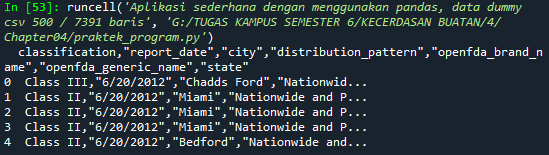
\includegraphics[scale=0.7]{figures/chappter4-1.png}}
		      \caption{Aplikasi Pandas - Chapter4}
		      \label{Aplikasi Pandas - Chapter4}
	      \end{figure}
	      \newpage

	\item dari dataframe tersebut dipecah menjadi dua dataframe yaitu 450 row pertama dan 50 row sisanya(harus beda dengan teman sekelas)
	      \begin{figure}[ht]
		      \centerline{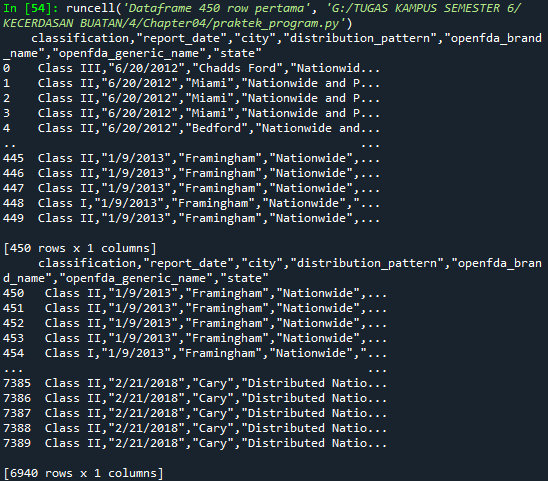
\includegraphics[scale=0.7]{figures/chappter4-2.png}}
		      \caption{Dataframe dipecah menjadi dua - Chapter4}
		      \label{Dataframe dipecah menjadi dua- Chapter4}
	      \end{figure}
	      \newpage

	\item pratekkan vektorisasi dan klasifikasi dari data (NPM mod 4, jika 0 maka katty perry, 1 LMFAO, 2 Eminem, 3 Shakira) dengan Decission Tree. Tunjukkan keluarannya dari komputer sendiri dan artikan maksud setiap luaran yang didapatkan.
	      \begin{figure}[ht]
		      \centerline{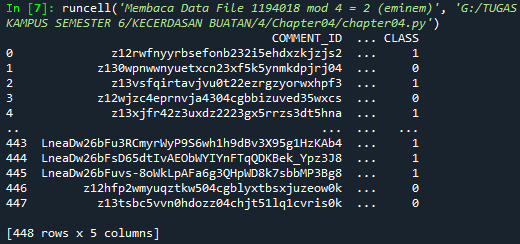
\includegraphics[scale=0.7]{figures/chappter4-3.png}}
		      \caption{Vektorisasi dan Klasifikasi 1194018 = mod 2 - Chapter4}
		      \label{Vektorisasi dan Klasifikasi 1194018 = mod 2 - Chapter4}
	      \end{figure}

	\item Cobalah klasifikasikan dari data vektorisasi yang di tentukan di nomor sebelumnya dengan klasifikasi SVM. Tunjukkan keluarannya dari komputer sendiri dan artikan maksud setiap luaran yang didapatkan.
	      \begin{figure}[ht]
		      \centerline{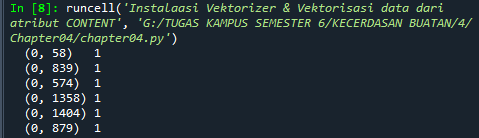
\includegraphics[scale=0.7]{figures/chappter4-4.png}}
		      \centerline{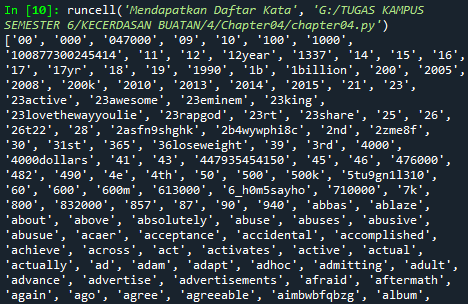
\includegraphics[scale=0.7]{figures/chappter4-4a.png}}
	      \end{figure}
	      \newpage
	      \begin{figure}[ht]
		      \centerline{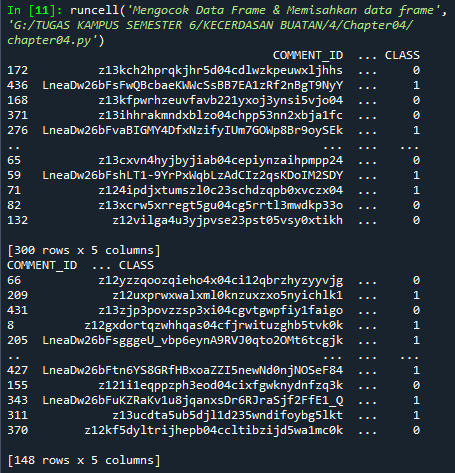
\includegraphics[scale=0.7]{figures/chappter4-4b.png}}
		      \centerline{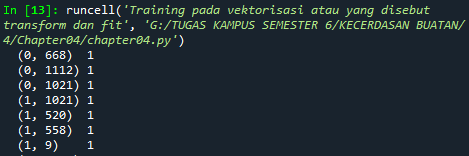
\includegraphics[scale=0.7]{figures/chappter4-4c.png}}
		      \centerline{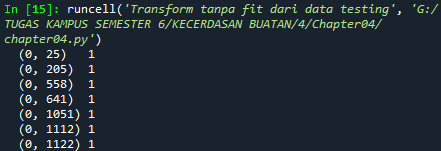
\includegraphics[scale=0.7]{figures/chappter4-4d.png}}
	      \end{figure}
	      \newpage
	      \begin{figure}[ht]
		      \centerline{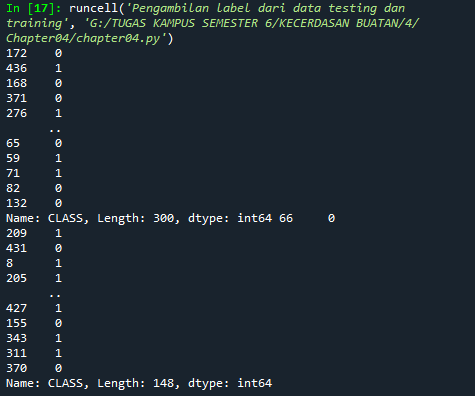
\includegraphics[scale=0.7]{figures/chappter4-4e.png}}
		      \centerline{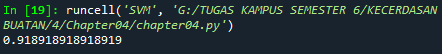
\includegraphics[scale=0.7]{figures/chappter4-4f.png}}
		      \caption{Vektorisasi dan Klasifikasi - Chapter4}
		      \label{Vektorisasi dan Klasifikasi- Chapter4}
	      \end{figure}

	\item Cobalah klasifikasikan dari data vektorisasi yang di tentukan di nomor sebelumnya dengan klasifikasi Decission Tree. Tunjukkan keluarannya dari komputer sendiri dan artikan maksud setiap luaran yang didapatkan.
	      \begin{figure}[ht]
		      \centerline{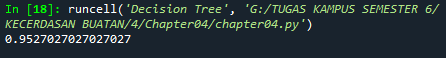
\includegraphics[scale=0.7]{figures/chappter4-5.png}}
		      \caption{Vektorisasi dan Klasifikasi Decission Tree - Chapter4}
		      \label{Vektorisasi dan Klasifikasi Decission Tree - Chapter4}
	      \end{figure}

	\item Plotlah confusion matrix dari praktek modul ini menggunakan matplotlib.Tunjukkan keluarannya dari komputer sendiri dan artikan maksud setiap luaran yang didapatkan.
	      \begin{figure}[ht]
		      \centerline{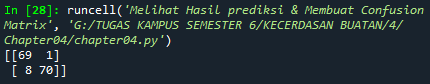
\includegraphics[scale=0.7]{figures/chappter4-6.png}}
		      \caption{Confusion Matrix - Chapter4}
		      \label{Confusion Matrix - Chapter4}
	      \end{figure}

	\item jalankan program cross validaiton pada bagian teori bab ini. Tunjukkan keluarannya dari komputer sendiri dan artikan maksud setiap luaran yang didapatkan.
	\newpage
	\begin{figure}[ht]
		\centerline{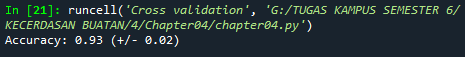
\includegraphics[scale=0.7]{figures/chappter4-7.png}}
		\centerline{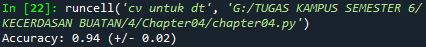
\includegraphics[scale=0.7]{figures/chappter4-7a.png}}
		\centerline{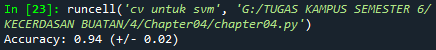
\includegraphics[scale=0.7]{figures/chappter4-7b.png}}
		\centerline{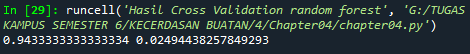
\includegraphics[scale=0.7]{figures/chappter4-7c.png}}
		\caption{Cross Validaiton - Chapter4}
		\label{Cross Validaiton - Chapter4}
	\end{figure}

	\item Buatlah program pengamatan komponen informasi pada bagian teori bab ini. Tunjukkan keluarannya dari komputer sendiri dan artikan maksud setiap luaran yang didapatkan.
	\begin{figure}[ht]
		\centerline{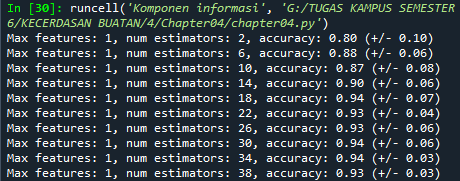
\includegraphics[scale=0.7]{figures/chappter4-8.png}}
		\centerline{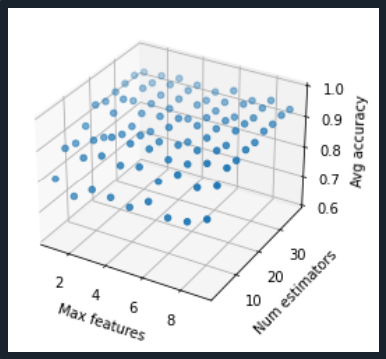
\includegraphics[scale=0.7]{figures/chappter4-8a.png}}
		\caption{Komponen Informasi - Chapter4}
		\label{Komponen Informasi - Chapter4}
	\end{figure}
\end{enumerate}


\section{Penanganan Error}
Dari praktek pemrograman yang dilakukan di modul ini, error yang kita dapatkan(hasil komputer sendiri) di dokumentasikan dan di selesaikan(nilai 5 per error yang ditangani. Untuk hari kedua):

\begin{enumerate}
	\item skrinsut error
	\item Tuliskan kode eror dan jenis errornya
	\item Solusi pemecahan masalah error tersebut
\end{enumerate}

\section{Presentasi Tugas}
Pada pertemuan ketiga ini, diadakan tiga penilaiain yaitu penilaian untuk tugas mingguan seperti sebelumnya dengan nilai maksimal 100. Kemudian dalam satu minggu kedepan maksimal sebelum waktu mata kuliah kecerdasan buatan. Ada presentasi kematerian dengan nilai presentasi yang terpisah masing-masing 100. Jadi ada tiga komponen penilaiain pada pertemuan ini yaitu :
\begin{enumerate}
	\item tugas minggu hari ini dan besok (maks 100). pada chapter ini
	\item presentasi Vektorisasi (maks 100). Mempraktekkan kode python dan menjelaskan cara kerjanya.
	\item presentasi cara kerja Data Frame di Pandas (maks 100).Mempraktekkan kode python dan menjelaskan cara kerjanya.
\end{enumerate}
Waktu presentasi pada jam kerja di IRC. Kriteria penilaian presentasi sangat sederhana, presenter akan ditanyai 20 pertanyaan tentang pemahamannya menggunakan python untuk kecerdasan buatan. jika presenter tidak bisa menjawab satu pertanyaan asisten maka nilai nol. Jika semua pertanyaan bisa dijawab maka nilai 100. Presentasi bisa diulang apabila gagal, sampai bisa mendapatkan nilai 100 dalam waktu satu minggu kedepan.


